\chapter{When a Loan Becomes a Business You Never Wanted}

A short interview can carry a complete theory of entrepreneurial risk if we read it carefully. The question is simple: what was the worst financial decision? The answer comes before the story: getting involved in something one does not want to be involved in. What follows is not a technical finance lecture with interest rates and loan-to-value ratios. It is a compact case study in how a deal that looked temporary and collateralized became an unwanted operating responsibility, then a catastrophic loss. This chapter follows the School of Hard Knocks interview, curated by LazyingArt LLC through Video2Book, and keeps the transcript as the source of truth.

\section{The Question and the Rule}

The opening question asks for the worst financial decision made over a lifetime. The speaker does not begin with a number, a market, or a formal investment category. He begins with a rule:

\begin{equation}
\text{bad involvement}
=
\text{entering a problem one does not want to own}.
\end{equation}

That equation is not a quotation from a board; it is a compact way to write the logic of the answer. The speaker's phrase is more direct: getting involved in things you do not want to be involved in. The important point is the order. The conclusion appears first, and the story is then used as evidence.

We should resist turning this into a generic maxim too quickly. In the transcript, the rule has a specific setting: a construction loan on a business he did not want to be in. That means the mistake is not simply that money was lost. The mistake is that the deal carried a form of responsibility he already knew he did not want.

\section{A Loan That Looked Bounded}

The concrete case begins with a construction loan. The speaker says he had the misfortune of doing such a loan on a business he really did not want to be in. He also says he was talked into it by a friend. That matters because it locates the decision between two forces: internal reluctance and external persuasion.

The loan appeared bounded in two ways. It was supposed to be temporary, and everything was collateralized. In ordinary business language, those are meant to reduce danger. A temporary loan is supposed to end. Collateral is supposed to stand behind the debt.

We can write the apparent structure as

\begin{equation}
E_{\text{nominal}}
=
E_{\text{capital under loan terms}},
\end{equation}

where \(E_{\text{nominal}}\) means the exposure one imagines when looking only at the stated financial instrument. But the speaker's story turns on the fact that this was not the whole exposure.

\subsection{Question \& Answer}

\paragraph{Question.}
If the construction loan was supposed to be temporary and collateralized, why did it become the speaker's worst financial decision?

\paragraph{Answer.}
Because a loan is not always just a loan. The stated risk may be financial, but the real risk can include being forced into the business when management fails. Collateral may reduce one kind of loss, and short duration may reduce another, but neither automatically removes time exposure, operating exposure, reputational exposure, or catastrophic event exposure.

The distinction is

\begin{equation}
\text{nominal loan risk}
\neq
\text{total entrepreneurial exposure}.
\end{equation}

This is the central mechanism of the interview. The deal was framed as a temporary construction loan, but the lived exposure became much larger than the initial frame.

\begin{table}
\centering
\begin{tabular}{p{0.28\linewidth} p{0.31\linewidth} p{0.28\linewidth}}
\hline
Promised protection & Hidden exposure & Transcript outcome \\
\hline
Temporary loan & Time and attention if the business fails & A couple of years spent turning it around \\
Collateralized deal & Operating responsibility beyond paper security & Management was failing \\
Bounded financing role & Tail risk attached to the business itself & Accident, death, company loss \\
\hline
\end{tabular}
\end{table}

\section{From Financing to Operating Responsibility}

The next movement in the story is the reversal. The company ended up with failing management. The speaker then had to step in and spend a couple of years turning it around.

This is the moment where the loan mutates. The nominal role is financier. The practical role becomes operator. A useful note-writing abstraction is to decompose total exposure into parts:

\begin{align}
E_{\text{total}}
&=
E_{\text{capital}}
+
E_{\text{time}}
+
E_{\text{operating}}
+
E_{\text{tail}}.
\end{align}

Only some of these terms are visible at the start of a deal. The capital exposure is usually the easiest to name. The time exposure appears when a supposedly passive investment begins to demand years of attention. The operating exposure appears when management failure forces intervention. The tail exposure appears when rare but severe events attach themselves to the business.

Here is the worked decomposition for this case, staying within what the transcript supports:

\begin{enumerate}
\item The initial reluctance is present from the beginning: the business is one he did not want to be in.
\item The apparent protection is the loan form: it was supposed to be temporary and collateralized.
\item The first hidden term appears when management fails:
\[
E_{\text{operating}} > 0.
\]
\item The second hidden term appears when he spends a couple of years turning the company around:
\[
E_{\text{time}} > 0.
\]
\item The final outcome includes a tragic accident, the loss of the company, and a reported personal loss close to
\[
L \approx \$3{,}000{,}000.
\]
\end{enumerate}

The arithmetic is not the point. The classification is the point. A decision that looked like a capital allocation became a claim on years of life and operating responsibility.

\begin{figure}
\centering
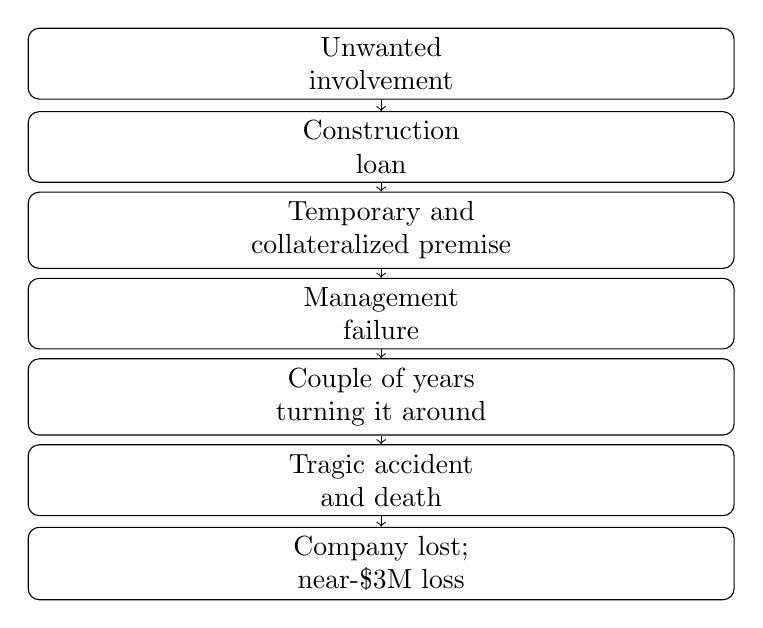
\begin{tikzpicture}[scale=0.92]
\node[draw, rounded corners, align=center, text width=0.72\linewidth] (a) at (0,0) {Unwanted\\involvement};
\node[draw, rounded corners, align=center, text width=0.72\linewidth] (b) at (0,-1.15) {Construction\\loan};
\node[draw, rounded corners, align=center, text width=0.72\linewidth] (c) at (0,-2.30) {Temporary and\\collateralized premise};
\node[draw, rounded corners, align=center, text width=0.72\linewidth] (d) at (0,-3.45) {Management\\failure};
\node[draw, rounded corners, align=center, text width=0.72\linewidth] (e) at (0,-4.60) {Couple of years\\turning it around};
\node[draw, rounded corners, align=center, text width=0.72\linewidth] (f) at (0,-5.75) {Tragic accident\\and death};
\node[draw, rounded corners, align=center, text width=0.72\linewidth] (g) at (0,-6.90) {Company lost;\\near-\$3M loss};

\draw[->] (a) -- (b);
\draw[->] (b) -- (c);
\draw[->] (c) -- (d);
\draw[->] (d) -- (e);
\draw[->] (e) -- (f);
\draw[->] (f) -- (g);
\end{tikzpicture}
\end{figure}

\section{The Tail Event and the Reported Loss}

After the turnaround effort, the story does not resolve into recovery. The speaker says the whole thing was affected by a tragic accident, and somebody unfortunately passed away. The business consequence, as he states it, was severe: it ended up costing the entire company.

We should not add facts that are not in the transcript. We do not know the legal structure, the insurance situation, the collateral value, the ownership arrangement, or the exact causal chain. The source gives us the sober outline: accident, death, company loss, and a personal loss close to three million dollars.

The transcript-backed endpoint is therefore

\begin{equation}
L \approx \$3{,}000{,}000,
\end{equation}

with the understanding that \(L\) denotes the reported personal loss, not a reconstructed balance sheet.

Placed in sequence, the whole exposure chain is

\begin{equation}
\text{reluctance}
\to
\text{loan}
\to
\text{failed management}
\to
\text{turnaround work}
\to
\text{tragic event}
\to
\text{company loss}
\to
L \approx \$3{,}000{,}000.
\end{equation}

This is why the opening rule is stronger than it first sounds. The objection at the beginning was not merely emotional. It was information about willingness to bear the full problem.

\section{The Decision Rule}

The closing lesson returns to the beginning. The speaker says the experience taught him not to get involved in something he does not want to get involved in. He adds that his gut instinct was telling him from day one not to do it, but he did it anyway.

A disciplined version of that rule is not simply ``trust your gut'' in the abstract. It is a screening rule:

\begin{equation}
\text{Reject the deal if }
E_{\text{total}}
>
W_{\text{own}},
\end{equation}

where \(W_{\text{own}}\) means one's real willingness to own the problem if the deal stops behaving according to its optimistic description. This is not a formula for pricing the loan. It is a formula for refusing a role.

In this interview, the speaker's unwillingness was known at the beginning. The later events revealed why that unwillingness mattered. If the downside of a transaction is that we become responsible for a business, crisis, or operating role we already know we do not want, then the protection offered by collateral and temporary terms may be inadequate.

\section{Summary}

The chapter's lesson is a small but serious piece of entrepreneurial reasoning. A deal can be financially bounded on paper and still personally unbounded in practice. The speaker entered a construction loan on a business he did not want to be in, partly through social persuasion. It was supposed to be temporary and collateralized. Management failed, he stepped in for a couple of years, a tragic accident followed, the company was lost, and he reports losing close to \( \$3{,}000{,}000 \).

The durable principle is this: before asking whether a deal is protected, ask whether the hidden downside would force us to own a problem we do not want. If the answer is yes, the real exposure is larger than the loan.